

Carl von Clausewitz famously described war as ``simply a continuation of political intercourse, with the addition of other means \parencite[605]{Clausewitz1989}.'' %
This statement has traditionally been used to remind the reader that
war is not an in itself, but a means to a political end. %
However, that insight is well integrated into current international relations theories of war. %
War is thought to consist of both bargaining and fighting, and the theoretical puzzle is why, given that war is costly, then why do states use this \textit{ex post} inefficient method to come to an agreement. %
But that is not the only puzzle regarding war. %
There are many such costly methods to use in bargaining, even delay is costly. %
The fundamental question of war is thus: Why war and not some other costly process. %
Stated another way, what is it that the ``additional means'' of military combat adds that allows the disagreement to be resolved through war but not through other means. %
Thus understanding what the ``additional means'' adds to politics requires understanding the nature of military combat, what \textcite{Gartner1998} calls ``opening up the black box of war''.

This paper proposes a quantitative case study method for studying war termination using financial market data. The prices of many financial asset are contingent on the outcomes of war. Because the payoffs of these assets are contingent on war outcomes, they can effectively serve as prediction markets of the war outcome, and provide a measure of expected war outcome. And because the prices of these assets are often observed at a high frequency, they can be used to measure changes in the expected war outcome within the war. Thus, although
detailed intra-war data may only be available for a single case, if
appropriate price data are available, the effects of war events on the
expected war outcome can be estimated. This paper builds on a large and
growing literature which measures impact or identifies important
political events using financial
\parencites{NorthWeingast1989}{north2000introd}{FreyKucher2000}{sussman2000instit}{wells2000revol}{Herron2000}{eldor2004finan}{ChenSiems2004}{Greenstone2007}
or prediction
markets \parencites{WolfersZitzewitz2004}{ArrowForsytheGorhamEtAl2008}{WolfersZitzewitz2009}.


How do financial markets respond to war events?
How do the events within war, such as battles, lead to the termination of war?
This paper addresses both of these questions by estimating the effects of battles in the American Civil War on the prices of Union bonds.
The strategy of this paper is to answer the first question in order to understand the second.
The credit risk of Union bonds was almost certainly driven by the expected debt of the Union.
The expected debt was driven by expectations of how the war would influence the size of that debt through expenditures and the resources to pay off that debt through its
Since military expenditures accounted for almost all Union expenditures and the price movements during the war were unprecedented, the changes in Union bond prices appear to be an indicator of the markets' expectations about how war events affected the expected war result.
Thus, events associated with large changes in the price of Union bonds can be used to infer those events which had large influences on the expected war result.

Financial assuet price data, through its relationship to the expected war result, a provides a proxy for war results with within-war variation that can be used to estimate the effect of events on the expected war result.


The prices of The prices of the financial are a summary (weighted
expectation, cite?) of the beliefs of the investors in that market
conditional on the data avaiable at the time. It is important to
reiterate that prices reflect the beliefs of investors, and not
necessarily the beliefs of the belligerents' governments. The
beliefs of the investors incorporate the public information, while
the beliefs of the belligerents' governments incorporate the public
information and private signals that the governments receive. Given
this, prices cannot easily be used to test the divergence in beliefs
between the belligerents.%
\footnote{Although not impossible if there are prices in the markets
of each belligerent, and these markets have sufficiently different
information sets. The difficulty is that the prices of most markets
is rarely secret. Thus information only received by market A can
partially incorporated by the market B after investors in market B
obeserve the prices in market A.} %

Since market prices do not reflect the beliefs of belligerents, what
do the beliefs of the investors represent? The first interpretation is
that beliefs of the market are a good estimate of the ``true''
estimate of the war outcome. To the extent that the market is
efficient, it is incorporating all available public information.%
% \footnote{However, since large-n studies also have ex post
% information, they may be more efficient. E.g. the difference between
% filtered and smoothed estimates in forecasting, $p(\theta |
% y_{1:t-1})$ and $p(\theta| y_{1:T}$.} %
In this case, the market beliefs may be directly compared with the
estimates of war termination from large-n studies. The market
aggregates individual investor estimates which come from previously
observed information and outputs.

The alternate interpretation of market prices are that they represent
the prior beliefs of the belligerents at time t. Even if the market is
not a particulalry good predictor of duration and outcome, it may be a
good estimate of the prior beliefs of the participants at all times.
If the belligerents' governments have all (or almost all) information
that is available to investors, then the beliefs of the investors is
equivalent to the prior beliefs of the belligerents. The belligerents'
posterior beliefs at a given time will be the prior beliefs (market
beliefs) plus any private signals received up through that point. In a
model without private information
To the extent that way in which investors and the belligerents process
data is correlated, i.e. they have similar misperceptions and
cognitive biases (which can be represented as common signals they
receive), market prices may be a more appropriate measure of duration
and outcome of the war than estimates derived from statistical models.


\section{Financial Markets and the Study of War?}
\label{bonds_battles:sec:barg-theory-war}

Given that war is bargaining process \parencite{Fearon1995}, the fundamental question of war is how the mechanism of military conflict resolves the differences between the belligerents that had prevented an agreement from being struck prior to the war.
Since \textcite{Fearon1995}, a series of papers developed the theory of how fighting and bargaining interact within war \parencites{FilsonWerner2002}{Slantchev2003}{SmithStam2004}{Powell2004}{LeventogluSlantchev2007}{LangloisLanglois2009}{WolfordReiterCarrubba2011}.
However, there has relatively been little empirical work that tests the implications of the bargaining theory of war with intra-war data, exceptions including \textcites{Goemans2000}{Ramsay2008}{Reiter2009}{Weisiger2013}{Weisiger2015}.
% Why intra-war data?
A primary reason for this for this relative absence of work is the difficulty of obtaining the necessary data to evaluate the implications of the bargaining theory of war.
While the secondary implications of the bargaining theory of war have been tested, the direct implications and the mechanisms of the theory require data on the belligerents' estimates of capabilities and resolve, and bargaining offers \parencite[32]{Reiter2003}.

Due to the lack of detailed data for many wars as well as concerns about the comparability of wars, using within case analysis is an appealing methodology for analyzing the effect of conflict on war termination.
Financial market data provides a measure related to a political science outcome of interest, the war termination, that varies within war.

Among these, data on intra-war combat events, namely battles, would appear to be the most readily available.
Yet, the existing data on battles is generally both poor quality and quantity.
As of yet, there exists no battle-level equivalent with the comprehensive datasets such as the Correlates of War \parencite{SarkeesWayman2010} or the Uppsala Conflict Data Program.
The only existing dataset of intra-war battles covering a large number of wars is CDB90 \parencite{cdb90}.%
\footnote{This is a revision of the HERO battle database.}
However, the quality of CDB90 is often criticized, major issues being its sampling strategy and inconsistent definitions of what constitutes a battle.
The later of these is as much a unresolved conceptual issue as it is the fault of the data collection effort.%
\footnote{See \textcite{BiddleLong2004} for a fair discusison of these critiques.}
Other political science papers using battle level data either extend CDB90 or use data from other sources, usually \textcite{Clodfelter2008}.
But these datasets are generally gathered for the specific research question of interest rather than a general purpose, maintained dataset of battles.
More recently, Long and Biddle have collected data on casualties and strengths of belligerents in major multi-party wars \parencite{CochranLong2014}.
More recently There has has been some major efforts at collecting event data for conflicts:
such as ACLED \parencites{RaleighLinkeHegreEtAl2010}, Empirical Studies of Conflict (\href{http://esoc.princeton.edu/}{ESOC}), and the Open Event Data Alliance.%
\footnote{\url{http://openeventdata.org}}

However, due to the lack of multi-war intra-war data, the preferred approach to the empirical study of the bargaining theory of war with intra-war data has been qualitative case studies\parencites{Reiter2003}[][Chapter 9]{Reiter2009}.
Examples of such qualitative case studies include  \textcite{Goemans2000} (WWI) and \textcite{Reiter2009} (multiple wars).
While there are some implications of the bargaining model of war that can be tested with within-case data, such as those regarding the offers made throughout the war, the use of within-case data prohibits the use of several key dependent variables of interest in these models---the cost, duration, and outcome of a war---since there is no variation in these variables within a single war.
Both \textcite{Reiter2009} and \textcite{Goemans2000} use changes in beliefs and changes in offers as their dependent variables in their cases.
% TODO: awkward section. expand.

% TODO: Paragraph on not being able to compare information and commitment easily

Financial market data provides an alternative method with which to analyze how intra-war events influence war termination.
This work gains some insights about the American Civil War through the interest rates on U.S. government bonds but these can be applied in a variety of contexts.
First, financial markets incorporate public, and perhaps private, information.
Thus financial markets are a measure of beliefs based on public information and can be used to understand how events in the war influence these beliefs.
For bargaining models of war, the beliefs of the decision-makers are of primary importance.
But financial markets may provide a baseline of the what beliefs can be formed based on public information.
Second, the financial markets are also pseudo-prediction market.
Where these predictions are reasonably accurate, estimating the effects of events on the changes in the predictions are a proxy for how these events would influence war outcomes.

The relationship between financial assets are of interest to the study of war for at least several reasons.
First, it is intrinsically interesting becuase it represents a cost of the conflict as well as a means of supporting the conflict.
Second, since some assets have payoffs contingent on war outcomes, and prices of assets represent an expectation about future payoffs, in some cases the prices of financial assets can act like a prediction market of war outcomes.
This work will focus on the later in order to understand which events within the war influence expectations about how the war will end.

\textit{General relationship between asset prices and war outcomes. What sort of assets? How they can relate to war outcomes?}

The prices of financial assets reflect war yields 


Four interpretations of prices and why they may be interesting for the study of war:

\begin{enumerate}
\item Intrinsically interesting
\item Beliefs of the market.
\item Suppose that the market is efficient.
\item Causal effects of the war.
\end{enumerate}

The price, and by extension bond yield, is an expectation about the future conditional on the information available at the time to the market (and approximately a value weighted average of their beliefs).
Consequently, differences in prices reflect new information that changes these expectations.%
\footnote{Apart from deterministic aspects of the change in price such as a bond getting closer to maturity or the payment of a coupon in the previous period.}
The problem is that models with prices as outcomes, with prices used as expectations
Prices have a causal interpretation, and behave similar to dynamic causal models, e.g. Blackwell
However, this depends on how
However, these dynamic causal model also rely on counterfactual models.

\begin{itemize}
\item Able to use single cases, and
\item If war is heterogeneous, then the predictions may be a better estimate of the effect than measures using other sources.
  Using a cross-section of wars uses other wars to generate the counterfactual.
\end{itemize}
Even if beliefs are disconnected from the war, then these beliefs are interesting in themselves.

Prices directly measure common beliefs, and respond to surprising events.
Although they cannot necessarily distinguish between theories of private information and commitment, it does provide information about which events within a war influence the beliefs of the market (and perhaps all contemporaries) about the aspects of the outcome of the war.
This information may be useful to either build more specific theories, or to test new theories that may distinguish between those theories.

The payoff of the asset should be related to war outcome.
In general, sovereign bonds of the belligerents in the war are often related to the war outcome.
These bonds can be related to war outcomes through both the cost and duration of the war and the settlement of the war.

\textcite{HaberMitchenerOosterlinckEtAl2015} focus on sovereign debt of parties in civil war.
Since if the civil war ends in the defeat of the rebel side, it is almost certain that it will default since in almost all cases governments do not honor rebel debt.
However, the effect outcome of war on the probability of the repayment of sovereign debt incorporates more factors than that, as it also incorporates the cost of the war and its duration.
This means that it may be difficult to separate out the effects of the result (victory, defeat), and the cost and duration of the war.\footnote{
  Though not impossible: multiple assets from different parties to the war may make this feasible.
  Alternatively, a strong model of the effects of these on the price may also allow for identification of different effects.
}
Although this may seem a downside to the use of many financial assets as measures of the expected outcome of wars, it can also be seen as a benefit.
The financial market effectively acts as a single measure which weights both the financial costs and benefits of the war discounted over time.\footnote{
  Consider, is it a victory if a country destroys its economy and a generation to gain a small piece of territory?
}
This is not the only way to measure war outcomes, but is useful in that it able to combine costs and benefits on the same scale, and consider both, something which measures od war outcomes in common datasets, e.g. COW, do not.

The war or events of interest should be the primary influence on changes in the price of the asset.
Since prices incorporate expectations about the future and there is a measure of randomness to combat, the issue with non-war related events, is not necessarily one of bias, but one of the variance of the estimate.
Even if the war events are uncorrelated with other events, and thus no omitted variable bias, if they represent a small proportion of the variation in the price of the financial asset, it will be difficult to use that financial asset as a proxy for the beliefs of interest.
This would not be an issue if the researcher were just interested in the effect of those events on the price itself, in which case it would mean that the effect sizes of the events of interest are small, but it is an issue if the price is to serve as a proxy for another concept of interest, in which case it means that the signal of the price is relatively low compared to the noise.


Prices are particularly useful for analyzing intra-war events for
several reasons.%
\footnote{See \textcite{WillardGuinnaneEtAl1996}, \textcite{north2000introd}, and \textcite{FreyKucher2000} for other  discussions on the use of price data to analyze historical events.} %
First, they incorporate only ex ante information. This distinguishes price data from sources such as participant accounts written after the fact or secondary sources \parencites[1001]{WillardGuinnaneEtAl1996}[][188]{FreyKucher2000a}.
Second, investors have strong incentives to be truthful in their assessments because their payoffs are tied to being correct.
This distinguishes prices from sources such as surveys or diaries of decisionmakers, which like prices have only the information available at the time, but which the decisionmaker may not reveal the truth for strategic or emotional reasons \parencite[57]{Reiter2009}.%
\footnote{Although the investors had their own preferences on the war,
  their investments seemed motivated by their preference for profits,
  \begin{quote}
    Sectional feeling often entered largely into the bull and bear
    contests in the Gold Room, and Union men and rebel sympathizers fought
    their battles sometimes, as much to gratify this as to make money.
    \textcite[7]{Cornwallis1879}
  \end{quote}
  \begin{quote}
    The heaviest speculative orders were sent from Washington and
    Baltimore, and next to these, from Louisville, Kentucky, owing to
    these cities being in close communication to the seat of war and the
    rebel lines; and the operators there, almost to a man, were "bulls"
    in feeling, and strong Secessionists.  But though seldom or never
    found selling "short" they were quick to sell out their "long" gold
    --- that is the gold they were carrying --- whenever the Confederate
    arms met with a reverse, and as quick to buy it back again when the
    market seemed to "touch bottom" \textcite[5]{Cornwallis1879}.
  \end{quote}
  \textcite[210]{Mitchell1903} writes,
  \begin{quote}
    Viewed in a broad way, it is therefore a serious
    mistake to look on the gold market as a place where a few gamblers
    were tossing the premium about to suit their selfish schemes; a much
    saner view is that it was the place where the community's estimate
    of the government's credit was visibly recorded. Here, as in other
    markets, those operators succeeded who forecast the future
    correctly, and men who tried to advance the price of gold when
    public confidence was increasing, or to depress it when confidence
    was on the wane, learned to their cost that they were not masters of
    the situation.
  \end{quote}
} %
Third, war can have a large influence on the payoffs of financial assets, so prices are likely to be highly responsive to war events.
Fourth, price data can be available at high frequencies, e.g. daily.
This is in contrast with documentary evidence which may be produced at lower frequency, or be missing for large sections of time \parencite[][57]{Reiter2009}. For example, in this data, the highest price series has daily data. 
The high frequency of price data makes it possible to analyze the effects of individual events in conflicts.
Fifth, price data are a quantitative summary of the investors' expectations, and thus more robust to the subjective interpretation of researchers. 
This distinguishes price data from documentary evidence which must be interpreted by researchers \parencite[][58]{Reiter2009}. 
The quantitative nature of the data makes it easier to analyze not only what events mattered in conflict, but the magnitude of those effects \parencite{north2000introd}.

None of this is to say that price data dominates other data sources.
Price data is simply another tool for researchers to use when analyzing conflict. It has several weaknesses, and is not appropriate in all cases.
First, prices do not directly measure the beliefs of the belligerents. Prices only incorporate public information, and do not incorporate the private information available to decisionmakers. 
This means that prices cannot be used to directly answer questions about the convergence in beliefs between belligerents.
However, it may be possible that many informational bargaining models of war could restated so that they have implications on changes in the expected outcome of the war conditional on public information.
Second, in many conflicts appropriate price data may not be available. 
In many areas in which researchers are most interested in understanding conflict, e.g. civil wars in developing countries, there may not exist an asset that is liquid enough to provide reliable estimates. 
Also, even for states with liquid and well-developed markets in normal periods, states often intervene in their own markets during war, distorting the price signals \parencite[12]{HaberMitchenerOosterlinckEtAl2015}. Finally, in any case in which prices are used, the researcher will need to apply substantive knowledge of the assets, investors, and conflict in order to map the prices into estimates of the political science quantities of interest.


\begin{figure}[htpb]
  \centering
  \usetikzlibrary{shapes,arrows,fit}
\tikzset{
    %Define standard arrow tip
    >=stealth',
    %Define style for boxes
    punkt/.style={
           rectangle,
           rounded corners,
           draw,
           text centered},
    rectouter/.style={
      draw,
      rounded corners
    },
    % Define arrow style
    pil/.style={
           ->,
           thick}
}
\footnotesize
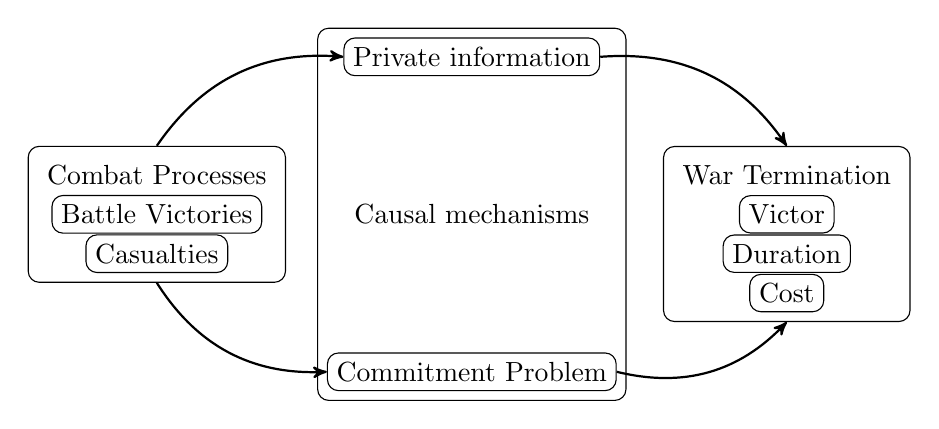
\begin{tikzpicture}[node distance=1cm, auto, scale=0.9]
  % Combat processes
 \node [] (combattitle) (combattitle) {Combat Processes};
 \node [punkt, below of=combattitle, node distance=0.5cm] (victory) {Battle Victories};
 \node [punkt, below of=victory, node distance=0.5cm] (casualties) {Casualties};
 \node [draw, rounded corners, fit={(combattitle) (victory) (casualties)}] (combat) {};

 % casual mechanisms
 \node [right of=combat, node distance=4cm] (dummy) {Causal mechanisms};
 \node [punkt, above of=dummy, node distance=2cm] (pi) {Private information};
 \node [punkt, below of=dummy, node distance=2cm] (cp) {Commitment
   Problem};
 \node [draw, rectouter, fit={(dummy) (pi) (cp)}] (causal) {};

 % war termination
 \node [punkt, right of=dummy, node distance=4cm] (wvictor)
 {Victor};
 \node [punkt, below of=wvictor, node distance=0.5cm] (wduration)
 {Duration};
 \node [punkt, below of=wduration, node distance=0.5cm] (wcost)
 {Cost};
 \node [above of=wvictor, node distance=0.5cm] (wterm)  {War Termination};
 \node[draw, rectouter, fit={(wterm) (wvictor) (wduration) (wcost)}] (end) {};

 % paths
 \draw [pil] (combat.north) to [bend left] (pi.west);
 \draw[pil] (combat.south) to [bend right] (cp.west);
 \draw[pil] (pi.east) to [bend left] (end.north);
 \draw[pil] (cp.east) to [bend right] (end.south);
\end{tikzpicture}
  \caption{Combat and War Termination}
  \label{bonds_battles:fig:combat-causal-diagram}
\end{figure}



\subsection{The Means and Mechanisms of War}
\label{bonds_battles:sec:means-mechanisms-war}

While I motivates the use of prices to study war beginning from bargaining theories of war, I do not attempt to directy test or distinguish between the private information and commitment theories of war.%
\footnote{See \textcite{Ramsay2008}, \textcite{Weisiger2015}, and \textcite{Reiter2009} for works which attempt to do so.}
Instead it will focus on the effect of military combat (victories and defeats in major battles) on the exptected cost of the war, without attempting to distinguish between informational and commitment theories.
This is because distinguishing between these theories using intra-war data is harder than previously appreciated.
Observing only battle results (victories or casualties) is insufficient to identify the casual mechanism of the war without some sort of strong model of the war process.
Models of which kind do not exist.
And models of which kind require deeper study of military processes, which this paper may in small part contribute.
This difficulty in identifying the effects of private information or commitment problems on war termination is an example of the general difficulty of identifying the causal effects of mediators \parencite{Keele2015a}.
This section explains the reasoning behind this claim.

War is the combination of a political bargaining process and a military combat process. %
\footnote{%
  ``Combat is a violent clash between at least two politically
  distinct groups organized to wield force. War consists of sustained
  and substantial episodes of combat.'' \parencite{Reiter2003} %
} %
These processes are distinct yet interrelated.%
\footnote{%
  For example, in costly process formal models of war, war is modeled
  as alternating round of ``bargaining'' and ``fighting''. %
  The bargaining and combat are distinct, but the outcome of the game
  depends on both. %
} %
It is the presence military combat that makes war distinct from other bargaining processes, and the bargaining that preceeds or succeeds it. %
Which leads to the primary puzzle in the study of war: What is the nature of the relationship between bargaining and the military combat? 
This raises the questions:
What are the frictions that prevented a negotiated agreement before war?
How did the actual fighting within war remove those frictions?
And why was fighting the only or preferred means to remove those frictions? 
There are two necessary components to understanding this puzzle. %
The first is the means of combat. %
The immediate goals of combat are the destruction of military forces, the destruction of civilian assets, or the control of territory.
\parencite[30]{Reiter2003}. %
The second is the causal mechanisms by which those means influence the bargaining process and war termination. %
Since a complete and coherent theory requires that combat solve the frictions that prevented a negotiated settlement without war \parencite{LeventogluSlantchev2007}, these causal mechanisms are the three rataionalist theories of war identified in \textcite{Fearon1995}: private information, commitment, and indivisibility. %
Thus there exist multiple possible means of combat and multiple channels by which each of those means may influence war termination.

Formal models can be classified by the casual mechanism by which combat influences war termination and by the means of combat. %
The formal models differ not only alter the mechanism in which they are interested (private information or commitment), but also the role of battles in the war, and the nature of the combat process: whether battles are important primarily because they impose costs (resolve), or because they can create war victory (probability of victory). %
Battle victory can bring total victory or collapse in war, either suddenly \parencites{Powell2004}{Wagner2000}{LeventogluSlantchev2007}, or over time \parencites{Slantchev2003}{SmithStam2004}. 
Battles also impose costs \parencites{FilsonWerner2002}{Powell2004}{LeventogluSlantchev2007}. %

The second approach, which is adopted in this paper, is to focus on which observable features of battles effect war termination, regardless of whether those effects occur through the private information or commitment problem channels. This appears in formal models as well. %
Bargaining is conditioned on the military combat process of war, and what would happen if that process continues to completion.

This bargaining is conditional on the state of that process or
expectations about the future state of that combat process.
\textcite[135]{Wagner2000} writes,
\begin{quotation}
  while states that are fighting may not actually try to disarm each
  other, they must bear in mind the fact that they could, and absolute
  way, even though it never occurs, must be the ``measure of all their
  hopes and fears.''
\end{quotation}

This approach is closer to earlier pre-bargaining empirical work on war (initiation) except in that it involves within war variables. %
The reason is that identifying the channel through which war events influences the end of war is empirically quite difficult. %
For almost any observable data of war outcomes, it both alters the actual state of the war and the beliefs of the participants about the combat process in which they are involved. %
And as of yet, there are no general results with empirical implications that differentiate between 

There are a couple ways in which this effects might be identified. %
First, if the beliefs of the participants were observed, then the effects of war events on the beliefs of the participants could be measured. %
One problem with this is that it is hard to observe the beliefs of the participants, even if diaries or reports are available, it is not clear whether these are accurate indicators of those beliefs. %
Another problem, is that it is insufficient to simply observe changes in the beliefs of one pariticipant over time, as in \textcite{Reiter2009}. %
The causal mechanism in informational theories of war is the \textit{convergence} of beliefs of the belligerents to a common distribution. %
This requires knowing the beliefs of both sides, both the mean and variance of those beliefs, or at the very least, the variance of prior distribution based on public information. %
By using documentary data, \textcite{Goemans2000} and \textcite{Reiter2009} are able to do this.
Second, identification would have to rely on a much more detailed model of military combat and war than exists now.
However, this would require more work along the lines of \textcite{Biddle2004}, which focus on generating models of military combat correct, even if these models are not directly tied to political variables.

This is not to abandon the bargaining theory of war or to claim it is useless. 
It is to argue that the current incarnation of the theory require a deeper understanding of the specifics of the bargaining process and the combat process in order to develop models with empirical implications.
And that understanding of the specifics of those processes does not spring like Athena fully formed from the head of Zeus, but will come from the study of wars, and developing stylized facts and empirical patterns which will serve as the assumptions of models.

Nor are the extant formal models of war particularly useful, or designed for empirical testing. %
The models are written at a high level, and the causal mechanisms are generally unobservable variables. %
They establish what sorts of explanations of war are complete, and what sorts of explanations and models are not (anarchy, balance of power, offense-defensive balance).
This is nontrivial, as \textcite{Fearon1995} ruled out a number of classes of explanations as having insufficient argument, and also established that war can explained within a rational framework, without relying on ex post irrationality or misperceptions of the participants. 
However, the parameters is the models have only a tenous mapping to the real world. %
The comparative statics in the models are generally determined by specific features of the bargaining framework and it is unclear whether these are general conditions. %
For example, there are claims that wars of information must be short based on \textcite{Slantchev2003} because in that model war can only last 3 rounds. %
However, that result is a direct result of the assumption that there are three types; increase the number of types (or the variance in the power of those types) and the duration of the war increases. %
\textcite{Powell2004} empirical implication is that wars of uncertainty about resolve are shorter than those of uncertainty about fighting. %
That result follows from the feature that costs are incurred between battles; but if costs can be incurred without fighting, and that is enough to allow for the resolution of combat, then why fight at all? 

Much of the discussion of models of war has discussed whether war is bargaining or commitment.
However, also important is the nature of the combat process that underlies the bargaining model. %
The difficulty is that these processes may be extremely hererogenous, across time and space \parencite{Reiter2003}.
But these are not reasons to ignore the processes, but patterns to be understood and explained. %
For while war may look different and be fought differently in time and
space, there must be similarities in it, or we would not call of those events ``war''. %
Moreover, understanding the different forms of the combat process is important to understanding how information and commitment problems are resolved through conflict. %
Better identifying the combat processes present in wars may provide different implications of those models, and thus make it easier to
distinguish when or if they are present.%
\footnote{%
  For example, \textcite{Walter2009} conjectures that insurgency is slower to reveal information than other forms of war. %
  Rigorously evaluating theories in this manner would require better theories of the actual military rationale between insurgency versus conventional war, the characteristics of each, and when belligerents choose to use each.
} %



\section{Why The American Civil War?}
\label{bonds_battles:sec:why-american-civil}

I chose the American Civil War as a case for the quality and quantity of its battle-level data, and the expected close relationship between government issued financial assets and war events.
In terms of its battle data, the American Civil War is one of the better documented wars, so quality battle-level is available.%
\footnote{%
  For example, \textit{The Official Records of the Union and  Confederate Armies} \parencites{US1901}, published between 1880 and 1901, consists of 128 books in 70 volumes totaling 139 thousand pages. %
} %
However, although there are multiple sources of American Civil War battle data, there has previously not been a comprehensive database suitable for quantitative analysis.

There is a long and deep economic history literature that documents the close relationship between war expectations and events and financial market prices during the American Civil War \parencites{Mitchell1903}{Mitchell1908}{Calomiris1988}{WillardGuinnaneEtAl1996}{McCandless1996}{SmithSmith1997}{Schwab1901}{Weidenmier2002}{BurdekinLangdana1993}{DavisPecquet1990}{BrownBurdekin2000}{OosterlinckWeidenmier2007}{Roll1972}.
I discuss why financial assets issued by the belligerents of the American Civil War may be particularly useful for understanding war in section \ref{bonds_battles:sec:why-prices-study}.

While the generalizability of this case is a function of its similarity to other cases, the American Civil War is more similar to modern civil wars than its 150 year age may suggest.
First, the American Civil War introduced several of the technologies later used in World War I and later, including rifled artillery, telegraph, machine guns, barbed wire, ironclad warships, and submarines.
The American Civil War is on the threshold of the era of modern warfare, if not the first modern war\parencites[89][]{Fuller1956a}[760]{Weiss1966}.%
\footnote{
  \begin{quotation}
    The Civil War was the first in which railroads were extensively used for the transportation of troops, aerial reconnaissance was effectively used, command and control was exercised through the electric telegraph, ironclad naval vessels engaged in combat, a multimanned submarine sank a naval vessel, rifled artillery came into general use, wire entanglements were used in field fortifications, and the repeating rifle was used by large troop units. \parencite[760]{Weiss1966}
  \end{quotation}
}
Second, the American Civil War was primarily a conventional war.
This places it in the plurality of post-Cold War civil wars, half of which are conventional war\parencite[423]{kalyvas2010inter}.%
\footnote{
  \textcite{kalyvas2010inter} notes that there is a ``striking decline [in] irregular wars following the end of the Cold War''.
}
Finally, the income levels of the Union and Confederacy in 1860 would place them as lower-middle income countries today---approximately the income levels of Pakistan and Iraq respectively.%
\footnote{%
  The GDP per capita of the US in 1860 was \$2,241 in 1990 GK international dollars. %
  In 2010, Cambodia had a GDP per capita of \$2,450, Pakistan \$2,494, and Ghana \$1,922 \parencite{BoltZanden2013}. %
  The southern states were poorer than the northern states, with a per capita consumption of about 70 percent of the overall U.S. level \parencite[324]{GoldinLewis1975}.
  The GDP per capita of the pre-war Confederacy is similar to that of Angola, Iraq and Senegal in 2010.%
  The estimated GDP per capita of the southern states in 1860 at 70\% that of the northern states was \$1,568. %
  In 2010, the following countries had approximately the same real GDP per capita: Angola \$1,600, Iraq \$1,610, and Senegal \$1,507 \parencite{BoltZanden2013}. %
}

The American Civil War is also an interesting case for study in its own right.
Its importance to American history is obvious, and need not be stated.%
\footnote{See \textcite{McPherson2003} among too many to list.}
But, given the voluminous literature on the subject, it is surprisingly understudied in two regards. %
First, the international relations literature has largely ignored the conflict.
Inter-state war scholars consider it a civil war, and intra-state war scholars focus on the post-1945 era \parencites[140-141]{Reiter2009}[2]{Poast2012}. %
Exceptions to this are \textcite{Reiter2009} and \textcite{Poast2012}.
Second, almost none of the existing work on the American Civil War, including the few examples in international relations, use any form of quantitative analysis.%
Consider, for example, that until \textcite{hacker2011census}, no historian had reanalyzed the total number killed in the American Civil War since \textcite{Livermore1900}.
There are a few previous examples of the analysis of American Civil battles from operations research, \textcite{Weiss1966} and
In applying international relations theory and quantitative methods to the study of this war, this work contributes a droplet to the ocean that is the literature on the American Civil War.



\section{U.S. Government Bond Yield Data}
\label{bonds_battles:sec:why-prices-study}



\subsection{The Fives of 1874}
\label{bonds_battles:sec:5s-1874}

This paper uses the long-run interest rate on government debt as a measure of expectations about the Civil War outcome.
The overall war outcome that is proxied by the interest rate of U.S. government debt almost certainly corresponds to expectatations about the cost and duration of the war rather than U.S. victory.
The yields of the 5's of 1874, a 5 percent coupon bond maturing in 1874, is the specific financial asset that is used as the the measure of long-run U.S. government interest rates.
The 5's of 1874 are used because they are the only U.S. government bond that was issued prior to the war and quoted throughout the war, meaning that it is the only time series from a single asset that has rates spanning the war.
This section expands upon these points.

As a measure of the long-run Union interest rate, this work uses the yield to maturity of the 5's of 1874.
The 5's of 1874 were a coupon bond issued under the authorization of the Act of June 14, 1858 to pay for a shortfall in funding due to the Panic of 1857.%
\footnote{See \textcites[p. 76]{Bayley1882}[78--79]{DeKnight1900}[42-43]{Treasury1863}[300-301, 305]{HomerSylla2005}}
As the name suggests, the 5's of 1874 were a coupon bond that paid 5 percent in specie (gold dollars) semi-annually on January and July, and were redeemable in 1874.
That the 5's of 1874 paid interest and principal in specie was important because on January 1st, 1862 the U.S. Treasury ceased redeeming notes in gold, and U.S. currency (Greenbacks) floated against gold until the resumption of convertibility on January 1st, 1879 \parencites{Dewey1918}{WillardGuinnaneEtAl1996}.

Firgures \ref{bonds_battles:fig:fives1874_price} and \ref{bonds_battles:fig:fives1874_yield} plot the price in gold dollars and yield to maturity of the 5's of 1874.
Prior to the war, the yield of the Fives was was low and had little variation, with its means between 4.5 and 5 percent.%
\footnote{
  This is actually below was generally considered risk-free rate in the U.S. for that period, 5 percent \parencite[][calls it the ``natural rate'']{Elder1863}.
  During this period British 3 percent consols had a yield of between of 3.10 and 3.28 \parencite[193]{HomerSylla2005}.
}
After Lincoln's election the interest rate rose to 6 percent, and after Sumter it rose to 8.2 percent.
During the war the interest rate fluctated between 5.2 percent and 14.7 percent, reaching its peak on July 30, 1864.
After surrender of Grant, the interest rate returned to stability with a rate higher than before the war, 6.5 percent.
These figures also plot the price
While the price and yields in terms of gold dollars fluctuated throughout the war, the price and yield in terms of currency (after January 1, 1862 when the Greenback floated against the gold dollar, were mostly stable.%
\footnote{See \textcite{Roll1972} for an analysis of this phenomena.}

The primary source of the prices of 5's of 1874 are tables of prices from the monthly financial trade publication published in New York, the \textit{Bankers' Magazine and Statistical Register}.
The \textit{Bankers' Magazine and Statistical Register}, along with the \textit{Merchants' Magazine and Commercial Chronicle}, was one of the major financial magazines of the period \parencites[186]{Mitchell1903}.
The prices of U.S. government and state bonds were quoted in tables, and the frequency of the quotes was approximately weekly.%
\footnote{
  Another monthly financial magazine, \textit{The Merchants' Magazine and Commercial Chronicle}, also published quotes for the 5's of 1874, but did not start publishing quotes of the prices of U.S. government bonds until January 1862, and stops quoting the 5's of 1874 in 1865.
  Thus paper relies on the series from the \textit{Bankers' Magazine and Statistical Register} because it quotes the 5's of 1874 over the whole period, 1861--1865.%
  This paper does not combine the quotes from the \textit{Bankers' Magazine} and \textit{Merchants' Magazine} because doing so would increase the complexity of the models. Using a single series keeps the data at approximately weekly frequency, and the larger gaps means reduces serial correlation.
}
The sources of the time quoted the prices of the bonds in currency.
To calculate the yield to maturity for the bond, the schedule of future cashflows is calcualated and converted to gold dollars using the current exchange rate of greenbacks to gold dollars and the expected depreciation of the gold dollar.%
\footnote{
  Since the price of bonds was quoted in currency but it paid interest and principal in currency, calculating the yields is difficult since they also incorporated beliefs about the future prices of gold dollars \parencites[Appendix A]{Macaulay1938}{Roll1972}{Calomiris1988}[302-303]{HomerSylla2005}.
  Most bonds, including the 5's of 1874, were priced in U.S. currency but paid specie and often principal in gold dollars.
  This paper accounts for this using a simple method to calculate the future price path of the dollar; it assumes that currency with appreciate at the risk free interest rate of 5 percent until it reaches parity with a gold dollar.
  This follows from an assumption that the risk free rate is constant over the period, and the gold dollar is priced as a risk-free zero-coupon bond with an unknown redemption date \cite{McCandless1996}.
  \textcite{Roll1972} and \textcite{Calomiris1988} estimate the expected depreciation of gold dollars in Greenbacks using differentials in bonds, however those methods cannot be applied to the period considered here.
}

The financial market data used in this work, as well as additional financial market data from the American Civil War period are provided in the dataset American Civil War Era Financial Data (ACWEFD) \parencite{Arnold2015a}.
ACWEFD contains bond prices and exchange rates published in the \textit{Bankers' Magazine} and \textit{Merchants' Magazine}, bid-level auction data, and miscellaneous financial and economic data for this period from a variety of primary and secondary sources.
The dataset is provided as an OKFN Data package with the source at \url{http://github.com/jrnold/civil_war_era_findata}.

The 5's of 1874 were not the only bond issued by the U.S. government during this period, but using this bond has several advantages when compared with other bonds.
The primary advantage of the 5's of 1874 was that it was the only coupon bond regularly quoted in the sources considered here throughout the war.
Additionally, unlike some other bonds issued during the war it was not callable by the government
The 6's of 1868, issued in 1848, was the other U.S. government bond issued prior to the war and quoted at the start of the war.
However, \textit{Bankers' Magazine} stops quoting in September 1861.
Another bond, the  6's of 1881 were issued under acts just prior to and at the start of the war, but they are not regularly quoted in the \textit{Bankers' Magazine} until September 1861.
The U.S. issued other bonds of various durations and rates throughout the war but they provide even shorter time series and in many cases contain options or were callable by the government.
\footnote{
The 5-20's and 10-40's were bonds callable by the government after 5 (10) years and redeemable in 20 (40) years.
The 7-30's were bonds that had coupon rates of 7.30 percent (2 cents per day), were redeemable in 3 years, but included the option to be exchanged for either the 6's of 1881 or 5-20's.
See \textcites{Bayley1882}{DeKnight1900}[297--309]{HomerSylla2005} for overviews of U.S. debt issues during this period.
}
Using the 5's of 1874 relative to other bonds should not make a substantive difference, since as Figure \ref{bonds_battles:fig:fives1874_union} shows, the yield to maturity of the 5's of 1874 is similar to the yields of all the other bonds issued by the U.S. government.
\footnote{
  While combining the various bond yields into a single issue could be more efficient, but would introduce other modeling complexities that I chose not to introduce in this work.
}
Several other analyses use the exchange rate between Greenbacks and gold dollars \parencites{McCandless1996}{WillardGuinnaneEtAl1996}{SmithSmith1997}.
The advantage of using interest rates relative to Greenbacks, is that since the Treasury department only issued Greenbacks after the war started and did not cease redemption for gold unil January 1862.
Thus while there are yields on the 5's of 1874 from April--December 1861, there no Greenbacks prices available during that period.
This is the period which should have the highest informational content in an informational theory of war, and includes battles such as the First Battle of Bull Run, and the Battle of Wilson's Creek.%
\footnote{\textcite{Poast2012} argues that the First Battle of Bull Run was pivotal in avoiding British recognition of the Confederate States.}
The choice of the U.S. government interest rates vs. greenback prices is unlikely to change the results here since the price of bonds in gold dollars closely follows the price of the Greenbacks in gold dollars, as shown in Figure \ref{bonds_battles:fig:fives1874_greenbacks}, and discussed in \textcite{Roll1972}.

The American Civil War is an ideal case in which to use prices to
infer expectations of war termination for three reasons. %
First, The war was of such severity that the fiscal policies of the
governments were essentially their military spending. %
The primary expense to the belligerents was the military. %
For the Union, the War and Navy Departments accounted for 86--96
percent of expenditures in the budget \parencites[][259]{Ball1991}[see
also][354-355]{BurdekinLangdana1993}. %
For the Union, the War and Navy Departments accounted for 76 percent
(in 1862) to 61 percent (in 1865) of the expenditures. %
The fraction of the budget spent directly on the military by the Union
was not due to a larger fraction spent on civilian matters, but due to
a larger fraction spent on servicing its debt, 20 (1862) to 36 (1865)
percent, the majority of which had been incurred to pay for the war.%
\footnote{%
  \textcite{Treasury1861a}, \textcite{Treasury1861b},
  \textcite{Treasury1862}, \textcite{Treasury1863}, and
  \textcite{Treasury1864} and \textcite{Treasury1865} %
} %
\parencite[][668]{McCandless1996} concludes ``During the war, the
single most important indicator of future government expenditures is
the process of the war itself.''%

Second, there is extensive historical and economic literature
establishing that war events are the single best determinant of bond
and currency prices during the American Civil War:
\parencites{Mitchell1903}{Mitchell1908}{Calomiris1988}{WillardGuinnaneEtAl1996}{McCandless1996}{SmithSmith1997},
graybacks \parencites{Schwab1901}{Weidenmier2002}, southern prices
\parencite{BurdekinLangdana1993}, Confederate bonds
\parencites{DavisPecquet1990}{BrownBurdekin2000}{OosterlinckWeidenmier2007},
and Union bonds \parencite{Roll1972}.%
\footnote{One notable exception is \textcite{BurdekinWeidenmier2001},
  which shows that the prices of graybacks in Richmond and Houston
  diverged due to differential application of monetary reform in late
  1864.}

Third, statements by and the actions of contemporary investors indicated the importance that war events had on the prices. %
Members of the government, military, and reporters all engaged in investment speculation based on their knowledge of war events \parencites[5-7]{Cornwallis1879}{Mitchell1903}[][1004]{WillardGuinnaneEtAl1996}.
Investment firms even had their own correspondents stationed in cities close to the war fronts to relay the latest news \parencites[5-7]{Cornwallis1879}. %
Magazines and newspapers often cited war events as the cause of recent price movements. %
For example, the issue of \textit{Bankers' Magazine} after Gettysburg and Vicksburg (Jul 23, 1863), cites these battles as the cause of the recent changes in market prices,
\begin{quote}
  The month of July has been a very active one with numerous fluctuations, almost daily, in the market values of gold, with unusual changes in the current values of stocks. %
  The advices as to the war movements are of a most satisfactory kind, leading to a fall in gold from 146 1/2 at the close of June, to 123 1/2, the 20th inst., at which dates the public had learned the  capitulation of Vicksburgh and of Port Hudson, the defeat of Lee in  Maryland and Pennsylvania, and of successful results at other points  for the Union forces. %
\parencite[159]{BankersMagazine1864}
\end{quote}



\subsection{U.S. Government Interest Rates are Primarily a Function of the Expected Cost of the War}
\label{bonds_battles:sec:u.s.-governm-inter}

When using prices or yields of a financial asset to proxy for expectations about a war outcome, it is necessary to identify which aspects of the war outcome that could influence the financial market.
The long-run U.S. government interest rates could be related to both expectations about the victor of the war and the cost of the war.
Using only the U.S. government interest rates and the  possible to disentangle these possibly cross-cutting effects of the expected war costs and outcome on bond prices.
However, it is likely that interest rates on U.S. government bonds mostly responded to expectations about the cost and duration of the war.

The fiscal position of the U.S. depended on the cost and duration of the war since the war was funded primarily through debt.
INSERT STATISTICS OF DEBT.
The future fiscal position of the U.S. also depended on victory in the war.
Reincorporating the seceeding states of the Confederacy back into the U.S. would increase the total resources from which the U.S. could repay its debts.
INSERT STATISTICS OF SIZE OF THE COFEDERACY.

Statements by government officials and market participants suggest more concern with the cost and duration of the war than with the inclusion of the Confederacy.
The economist, William Elder, in an 1863 analysis of the ability of the U.S. to repay its debt reprinted in the \textit{Bankers'  Magazine} claimed ``The Rebellion leaves our capital in real and personal property just where it was before the secession. \dots{} So far now this is only a loss of that which we have not had, and at best or worst, a very small one in any time of need'' \parencite[19]{Elder1863}.
The \textit{Annual Report of the Treasury Department} in 1863 noted,
\begin{quote}
It will not escape observation that the average [interest] rate is now increasing, and it is obvious that it must continue to increase with the increase of the proportion of the interest-bearing to the non-interest-bearing debt.
And as the amount of the latter, consisting of United States notes and fractional currency, cannot be materially augmented without evil consequences of the roost serious character, the rate of interest must increase with the debt, and approach continually the highest average.
That must be greater or less in proportion to the duration and cost of the war. \parencite[13]{Treasury1863}
\end{quote}

Comparing the time series of U.S. government interest rates to those of the Confederate currency and Northern and Southern States in Figure \ref{bonds_battles:fig:fives1874_compared} suggest that it is primarily driven by expectations of the cost of the war.
The bond yields of the Northern States which are almost certainly driven by costs of the war and possibly less dependent on victory since taxes would not necessarily go to pay off their debts are similar to that of U.S. government bonds.
However, the price of the Confederate currency follows a noticeably different pattern, almost decreasing monotonically over the entire course of the war.
Although some of this was due to an expansion of the monetary supply, the prices of Confederate bonds issued in Amsterdam and redeemable in gold also followed a similar pattern.
The prices of the Confederate currency and bonds almost certaintly was primarily driven by expectations about whether the Confederacy would retain sovereignty.
Thus, since the U.S. government interest rates do not follow an inverse pattern, means that they must be reflecting other factors, namely the cost of the war.

Another desirable aspect of using a financial asset to proxy expectations about a war outcome is that factors other than the war do not have much influence on its price or yield.
Non-war factors almost certainly had minimal, if any, effect on the long run interest rates of long-run U.S. government debt (at least relative to the war) because the war accounted for the overwhelming majority of the U.S. government expenditures during the war, and U.S. government bond prices in the years prior to the war were relatively stable.
The intensity of the American Civil War ensured that it was only important factor for the expectations about the U.S. government fiscal situation.
In the years 1862--1865, the War and Navy Departments of the government together accounted for between 76 percent (in 1862) to 61 percent (in 1865) of U.S. government expenditures.
Most of the remaining expenditure was debt financing, which accounted for 20 (1862) to 36 (1865) percent of expenditures, and the majority of which had been originally incurred to pay for war expenditures.%
\footnote{See also \textcite[][14]{Godfrey1976}.}
The budgetary effect of the war is clear when looking comparing estimates of the U.S. budget for fiscal year 1866 made before and after the war had ended.
In \textit{The Annual Report of the  Treasury} on December 6, 1864 the forecast deficit of the fiscal year ending June 30, 1866 was \$470 million, with 1,168 million in expenditures \parencite[13][]{Treasury1864}.
In the Annual Report of the Treasury issued on December 1865, the first after the conclusion of the war, the Treasury estimated a surplus of \$112 million, with expenditures of only \$396 million dollars \parencite{Treasury1865}.%
\footnote{There was a surplus of \$132 million for FY 1866 \parencite[2][]{Treasury1866}.}
The importance of the war on interest rates can also be seen in a comparison of interest rates prior and during the war.
Thus the variation seen during the war is certaintly entirely due to changes in expectations stemming from events within the war.
However, that is not to say that the important war events are battles, something which is addressed in Section \ref{bonds_battles:sec:battle-data}.

In summary, the interest rates of U.S. government bonds reflected some combination of expectations about the cost, duration and victor of the war.
However, it is more likely that they are largely reflecting expectations about the cost and duration of the war.

\begin{figure}[!]
  \centering
  \begin{subfigure}[b]{\linewidth}
   \includegraphics{../bonds_and_battles//paper/figure/fives1874_price-1}
  \caption{Price in gold dollars. Par value is \$100.}
  \label{bonds_battles:fig:fives1874_price}
\end{subfigure}
\begin{subfigure}[b]{\linewidth}
   \includegraphics{../bonds_and_battles//paper/figure/fives1874_yield-1}
  \caption{Yield to maturity.}
  \label{bonds_battles:fig:fives1874_yield}
\end{subfigure}
\caption[Price and yield of the 5's of 1874, 1858-1865]{Price and yield of the 5's of 1874 from its issue in 1858 until the end of the Civil War in 1865.
The yield is steady at near 5 percent until the election of Lincoln and the secession of the Southern States in late 1860-early 1861.
During the American Civil War, the yields are variable, spiking in the middle of 1864.
 }
\label{bonds_battles:fig:fives1874_yield_price}
\end{figure}

\begin{figure}[!]
  \begin{subfigure}[b]{0.45\linewidth}
    \includegraphics{../bonds_and_battles//paper/figure/fives1874_greenback_price-1}
  \caption{Price in gold dollars for the 5's of 1874 compared to the price of Greenbacks, 1862-1865.}
  \label{bonds_battles:fig:fives1874_greenbacks}
\end{subfigure}%
\hspace{0.1\linewidth}%
\begin{subfigure}[b]{0.45\linewidth}
    \includegraphics{../bonds_and_battles//paper/figure/fives1874_union-1}
  \caption{Yield to maturity of the 5's of 1874 compared with other U.S. bonds.}
  \label{bonds_battles:fig:fives1874_union}
\end{subfigure}

\begin{subfigure}[b]{0.45\linewidth}
  \centering
  \includegraphics{../bonds_and_battles//paper/figure/fives1874_north-1}
\caption{Yield to maturity of the 5's of 1874 compared with bonds issued by Northern states.}
\label{bonds_battles:fig:fives1874_north}
\end{subfigure}%
\hspace{0.1\linewidth}%
\begin{subfigure}[b]{0.45\linewidth}
  \includegraphics{../bonds_and_battles//paper/figure/fives1874_south-1}
\caption{Yield to maturity of the 5's of 1874 compared with bonds issued by Southern and border states.}
\label{bonds_battles:fig:fives1874_south}
\end{subfigure}

\begin{subfigure}[b]{0.45\linewidth}
  \includegraphics{../bonds_and_battles//paper/figure/fives1874_graybacks-1}
\caption{Price in gold dollars of the 5's of 1874 compared with \$100 Graybacks (Confederate currency).}
\label{bonds_battles:fig:fives1874_grayback}

\end{subfigure}
\caption[The 5's of 1874 compared with other government and states issued bonds and currency.]{The 5's of 1874 compared with other government and states issued bonds and currency.
  The 5's of 1874 follow a similar pattern as that of other U.S. bonds and those issued by Northern states.
  They diverge and have a different pattern than the Confederate currency and bonds issued by Southern states.
}
\label{bonds_battles:fig:fives1874_compared}
\end{figure}



\section{Battle Data}
\label{bonds_battles:sec:battle-data}

A theoretical and practical issue in the quantitative study of war is how to quantify and measure combat within wars.
There are, at least, two issues. 
The first issue is what to use as the unit of obervation: events or time periods.
Some work uses events, such as battles or campaigns, as the unit of observation \parencites{ReiterStam1998}{ReiterStam2002}{Ramsay2008}{PilsterBoehmelt2011a}{GrauerHorowitz2012}, while other work prefer values aggregated over time periods, e.g. such as monthly casualties \textcite{Weisiger2015}.
A second disagreement is over how to measure military suceess --- battle outcomes or casualties.
Some work uses victory or defeat in battle \parencites{ReiterStam1998}{ReiterStam2002}{GrauerHorowitz2012}, while other work uses casualties \parencites{Biddle2004}{BiddleLong2004}{PilsterBoehmelt2011a}.
In this work, I will use a set of ``militarily significanct'' battles in the American Civil war and their outcomes (Confederate or Union victory).
A key advantage of this method is that it allows me to estimate the effects of individual battles, as well as the average effect of Union and Confederate Victory.

The set of American Civil War battles used in the analysis is the set of the battles that the National Park Service Civil War Sites Advisory Commission (CWSAC) defined as the militarily significant in the war --- ``having a decisive influence on a campaign and a direct impact on the course of the war'' \parencite{CWSAC1993}.
Table \ref{bonds_battles:tab:battles} lists these battles.
These data come from a 1993 National Park Service report, ``Civil War Sites Advisory Commission Report on the Nation's Civil War Battlefields'' \parencites{CWSAC1993}{CWSAC1993b}.
The CWSAC was established by a 1990 law to preserve Civil War battlefields and was ``asked to identify the nation's historically significant Civil War sites; determine their relative importance; determine their condition; assess threats to their integrity; and recommend alternatives for preserving and interpreting them.'' \parencite{CWSAC1993b}
This report identified 383 battles militarily significant battles from the over 10,000 officially recorded engagements in the war.
Of the over 10,500 military engagements listed in the \textit{Official Records of the American Civil War}, CWSAC selected 384 battles as the ``principal batltes'' based on ``military significance''. 
\begin{quote}
  These sites encompass virtually all of the principal land battles that were of special strategic, tactical, or thematic importance to local operations, campaigns, theaters, or to the war as a whole \dots{} he more than 10,500 conflict sites excluded from our inventory were relatively unimportant as individual military actions. These conflicts were the venues and actions that implemented the war between and beyond the dramatic major engagements. \parencite{CWSAC1993}
\end{quote}
These principal battles were further classified into four categories according to their military and historical significance; A (``having a decisive influence on a campaign and a direct impact on the course of the war'') to D (``having a limited influence on the outcome of their campaign or operation but achieving or affecting important local objectives'').
This work will use 42 battles with the military significance classification of ``A'', listed in Table \ref{bonds_battles:tab:battles}.%
\footnote{
  Three CWSAC class ``A'' battles are omitted.
  The Batle of Fort Sumter (SC, April 12--14, 1861) is omitted because it marks the start of the war and the analysis starts after this battle.
  Given the small size of Fort Sumter, no casualties, the effects of the battle can be attributed to marking the start of conflict.
  The Battle of Fort Blakely (AL, April 2--9, 1865) is ommitted because news of battle does not reach New York City until after news of the surrender of Gen. Robert E. Lee's forces at Appomattox Court House on Apr 10, 1865.
  The Battle of Five Forks (VA, April 1, 1865) is omitted because I could not find reports of it in the \textit{New York Times}; news of it was overshadowed by that of other Battles, namely the Battle of Third Petersburg on April 2nd.
}
While this is a subset of the battles, it is still a relatively large number of battles by most war standards and similar in number and composition as the list of battles in other sources: \textcite{Livermore1900}, \textcite{Bodart1908}, \textcite{cdb90}.
So although this is the may be considered a subset of battle of the American Civil War, that is largely due to the completeness of the records and richness of the data on the American Civil War.

\begin{figure}[htpb]
  \centering
  \includegraphics{../bonds_and_battles//paper/figure/fig_major_battles-1}
  \caption{Major battles and their outcomes}
  \label{bonds_battles:fig:major_battles}
\end{figure}

The CWSAC report \parencite{CWSAC1993b} also classifies battles into ``Union victory'', ``Confederate victory'', and ``Inconclusive''.
While \textcite{CWSAC1993} does not describe the methodology used to classify the battle outcomes, the classifications largely argee with other sources \textcite{fox1898regimental}, \textcite{Livermore1900}, \textcite{Bodart1908} and \textcite{cdb90}.%
\footnote{\textcite{fox1898regimental} and \textcite{Livermore1900} are cited as sources for CWSAC.}
Two of those sources, \textcite{fox1898regimental} and \textcite{Livermore1900}, provide more description of their methodology for assigning victory --- the victorious side of a battle as the side that controls the battlefield at the end of battle.
The data consist of 29 Union victories and 13 Confederate victories and no ``Inconclusive'' battles.%
\footnote{
  Of the battles considered here, CWSAC classified two as ``Inconclusive'': The Wilderness, and Spotsylvania Court House.
  Since there are too few inclusive battles to get an estimate of their average effect, The Wilderness was reclassified as a Union victory, and Spotsylvania Court House as a Confederate victory based on how the results were reported in the news.
}
Figure \ref{bonds_battles:fig:major_battles} plots the date and outcomes of the  battles over time.
While CWSA

\begin{table}
  \centering
  \input{../bonds_and_battles//paper/tex/tab_major_battles.tex}
  \caption{List of the 42 major battles of the American Civil War included in this analysis.}
  \label{bonds_battles:tab:battles}
\end{table}

In order to estimate the effects of these battles, I need the time at which the New York markets learned of the outcomes.
In general, markets learned of the outcomes of battles relatively quickly:
\begin{quote}
Members of both Houses [of Congress], and of all political creeds, resident bankers, the lobby agents, clerks, and secretaries, haunted the War Department for the latest news from the seat of war.
The daily registry of the Gold Room was a quicker messenger of successes or defeats than the tardier telegrams of the Associated Press. A private secretary of a high official, with no capital at all save his position, which gave him authentic information of every shaping of the chess game of war a full twenty hours in advance of the public, simply flashed the words ``sell, buy'' across the wires, and trusted to the honor of his broker for the rest. \parencite[245]{Medbery1870a}\footnote{Originally quoted in \textcite{WillardGuinnaneEtAl1996}.}
\end{quote}
However, there was still a lag between the occurence of the battle, and when news of the outcome, and this lag varied with the distance of the battle from New York and Washington, as well as idiosyncratic circumstances.
As a measure of when information of the battle reaches the New York market, I coded an indicator for when news of the battle outcome in the \textit{New York Times}.%
This was not necessarily one day, for some battles (Chattonooga) which lasted several days of approximately equal intensity, I coded news reaching the market on several days.
However, for sieges which could last many days, \textit{e.g.} Vicksburg, Port Hudson, I only coded when news of the end of the siege was reported.
While battles the Eastern theater were reported on the same or next day (Antietam, Gettysburg), news on battles in other theaters may not reach the market for days.
The battle with the longest lag in news was the Battle of Glorietta Pass in New Mexico; it ended on March 28, 1862, but news of the battle did not reach New York city until April 15.
A data driven approach to identifying the timing of this news is important since in a time series analysis, the timing of the events is the primary factor in identifying their effects.
% Illustrative anecdotes: McClellan in Peninsula campaign, Sherman in march to the sea.

In using a small set of battles based on a \textit{ex post} expert assessment of their military importance, it is important to note that this is not selecting on the dependent variable.%
\footnote{
  That would be including explanatory variables by selecting periods of times that had large changes in yields. 
}
I am selecting a set of covariate, battles, which based on prior information are expected to have larg effects on the response variable.
This is no different than any other regression model, in which only a small set of covariates are selected of all possible variables in the universe, because those covariates are \textit{a priori} expected to plausibly have effect on the response variable.
By selecting a small number of battles, I take a dense problem, the effects of all possible events and military engagements, and turn it into a sparse problem, in which only a small number of battles potentially having a non-zero effect.
In doing so, I am able to etimates different effects for each battle.
With a larger number of battles, it would be necessary to pool the effects of battles, for example, all battles with the same casualties have the same effect.
But that may not sufficiently account for the context of battle.

Thus far, I have only discussed battles in this section, but battles not the only relevant events in a war, and this war in particular.
Changes in policy, leadership, foreign policy events, negoatiations and other events may all influenece expectations about the future of the war.
This paper does not include them in its models for two reasons. 
The first is that it is difficult to coherently choose a set of events. 
\textcite{McCandless1996} and \textcite{SmithSmith1997} both include lists of indicator variables for \textit{ad hoc} lists of military, fiscal, and political events in the war.
However, there is no clear rule as to what constitutes major non-battle events in the war, and what does not.
The list in \textcite{SmithSmith1997} does something similar to selecting on the dependent variable, by using events mentioned in \textcite{Mitchell1903} as corresponding to large daily movements in the market.%
\footnote{
  An exception to this is funding bills, where their effect can be modeled as a function of how much each bill increases the debt.
  The difficulty of including funding bills is the effect on the market should not occur when the bill is signed, which is easy, but during the negotatiations of the bill when information about the possible outcome of the vote is known.
}
The second reason is that non-battlefield events are more likely influenced by battlefield events than vice versa. 
For example, the capture of Atlanta is given as a reason why Linconln won the election of 1864.
The outcomes of battles influence expectations about the entire future course of the war, including non-battle events. 
Thus, the effects of the non-battle events on the prices and yields of financial assets is only the surprising part, only the events that are not anticipated given the previous events on the battlefield.
Since I do not include data on non-war events in the war, in the models of Section \ref{bonds_battles:sec:model-war-events} I will account for these events using fat-tailed distributions (Student's $t$) in the error term to allow for the effects of large events, although they are not included explicitly.
In Section \ref{bonds_battles:sec:conclusion}, I propse a more coherent method for identifying war and non-war events.

For this project, I created a public database of American Civil War battles, the American Civil War Battle Database \parencite{Arnold2015b}.
The American Civil War Battle Database combines, cleans, cross-references battle data from multiple primary and secondary sources, including \textcites{Phisterer1883}{Livermore1900}{Bodart1908}{dyer1908_war_rebel}{KennedyConservation1998}{CWSAC1993}{cwsac2012}.
This is the most complete, machine-readable data on American Civil War battles of which I am aware.

\section{Model of War Events on Yields}
\label{bonds_battles:sec:model-war-events}

Let $y_{i}$ be the natural logarithm of the yield.
The observations of $y$ are indexed by observation rather than time, because some adjustments are needed to account for the fact that yields are observed are irregular frequencies (between XXXXX and XXXX days).
$t[i] \in 0, \dots, T$ of observation $i$.
The model is a regression on the difference of the yields on covariates.
\begin{equation}
  \label{bonds_battles:eq:1}
  \begin{aligned}[t]
    y_{i} - y_{i - 1} &= \mu_{i} + \epsilon_{i} & \epsilon_{i} & \sim N(0, (t[i] - t[i - 1]) \sigma^{2}) \\
  \end{aligned}
\end{equation}
where $t[i] - t[i - 1]$ is the difference in days and is needed to account for the irregular spacing of observations.

The expected value of the difference in log yields, $\mu$, includes a constant respresenting a drift term, and the sum of the battle effects for those battles occuring during that time period,
\begin{equation}
  \label{bonds_battles:eq:2}
  \begin{aligned}[t]
    \mu_{i} &= \sum_{k = t[i-1] + 1}^{t[i]} \sum_{b \in B} w_{b,k} \beta_{b}
  \end{aligned}
\end{equation}
where $B$ is the set of battles.
The effect of a battle in a period is the sum of the product of a daily weight term $w_{b,k}$ ($\sum_{t \in 1:T} w_{b,t} = 1$) and its overall effect $\beta_{b}$.
The weight terms are equally weighted for each battle and non-zero on the 1st day(s) in which news of the battle was reported and a lag of XXXX days.
For example, the end of Gettysburg was reported in the news on XXXX, so XXXXX through XXXX (XXXX days later) have a weight of XXXX, and all other days have a weight of 0.

The effects of battles are modeled as coming from two distributions: Union victories, and Confederate victories.
\begin{equation}
  \label{bonds_battles:eq:4}
  \begin{aligned}[t]
  \beta_{b} &\sim
  \begin{cases}
    N(\gamma_{\mathtt{U}}, \zeta^{2}) & \text{if $b$ is a Union victory} \\
    N(\gamma_{\mathtt{C}}, \zeta^{2}) & \text{if $b$ is a Confederate victory}
  \end{cases}
  \end{aligned}
\end{equation}
This model allows for the estimation of the average effect of Union and Confederate victories ($\gamma$) while allowing for the effects to vary between battles and by extension over time.
The distributions share a common scale, $\zeta^{2}$, since there is not enough data to estimate separate scales well.

The posterior distribution of the was sampled with MCMC using the NUTS-HMC algorithm as implemented in Stan.
Convergence was asssessed using multiple chain $R$-hat.

\begin{itemize}
\item Average effect of victories and defeats.
\item Model comparison to naive version: WAIC.
\item Plot effects with and without war
\item Individual effects of battles.
\end{itemize}


In the analysis of the interest rates, the risk free interest rate and inflation are often included; in this work they will not be included.
Inflation is not included for several reasons.
First, while inflation measured in Greenbacks rose during this period, since the price of gold tracked the price of commodities during this period, inflation in terms of gold dollars was low\parencites{Mitchell1903}{Mitchell1908}. 
Second, even if that were not the case, the influence of the war was such that inflation would likely be considered a post-treatment variable that was responding to war events.
Third, the best measure of inflation, the Warren-Pearson Wholesale Price Index, is only available at the monthly level.
The risk free interest rate during this period is not used because it is hard to define one during this time \parencites{HomerSylla2005}.
In later periods, U.S. government bonds would be considered a risk free interest rate.
But this work uses U.S. government bonds precisely because they are risky with that risk varying with expectations of the war outcome.
\textcites{Macaulay1938}{HomerSylla2005} consider two other bond indexes as risk free interest rates: railroad bonds and New England municipal and state bonds.
During this period, railroad bonds were still relatively risky during this period, and had higher yields than U.S. government bonds.
Municipal bonds, when their yields are calculated in gold dollars, have yields similar to those of U.S. government bonds, and thus were not much less risky.
Additionally, the only available source of these interest rates, \textcite{Macaulay1938}, provides these interest rates at a monthly (railroad) and quarterly (New England municipals) frequency.
Other work in 19th century economic history use the interest rate of British consols is used as a risk free interest rate.
This is inappropriate for this analysis because that risk free interest rate was for the London market, and not the New York market.

\section{Conclusion}
\label{bonds_battles:sec:conclusion}

Use conclusion to outline issues with existing event studies, and how to address them using text as data.

\begin{itemize}
\item The first issue is the lag of events.
  When considering the effect of events on markets, it is not the time of the event \textit{per se} that is important, but the time at which \textit{information} about the event reaches the market.
  This can be handled through modeling --- e.g. estimating the lag structure, allowing for different different lags around events.
  However, these modeling strategies often implicitly rely on homogeneity of the lag across events to identify the effect.
  It can become difficult when there is heterogeneity in events. For example, the results of many battles in Virginia were known the next day, but the results of the Battle of Gloria Pass were not known until x.

\item The second issue is in confounding variables.
  This can be handled by including other variables and dummy variables for events in the analysis.
  But how does one handle the inclusion of these in a principled manner, especially when there are \textit{sui generis} events like the Emancipation Proclamation in the data?
\end{itemize}

Newspaper articles provide a means to address these concerns.

The analysis would consist of extracting events or topics from newspaper articles and estimating the effect of these extracted events on changes in prices.
This makes the assumption that the newspaper articles sufficiently reflects the information available to the market, which may seem extreme, but seems less problematic than the issues discussed earlier.
The importance of events relative to other events is identified through their prominence in the newspaper. E.g. if the front page is about a battle, then it is probably the news that is moving the market, whereas if the frontage is about a bill or the economy, then that is probably the more important news.

%%% Local Variables: 
%%% TeX-master: dissertation.tex
%%% End:
